% -*- coding: UTF-8 -*-
% vim: autoindent expandtab tabstop=4 sw=4 sts=4 filetype=tex
% vim: spelllang=de spell
% chktex-file 27 - disable warning about missing include files

\section{Modelle zur Schattierung (shading models)}
\label{sec:shading}

Sofern im Text nicht anders vermerkt, basieren die nachfolgenden
Abschnitte auf~\cite[S. 734–739]{foley_computer_1996},
sowie~\cite{hughes_computer_2013}.

Bei der Anwendung von Modellen zur Schattierung (\textit{shading
models}) geht es grundsätzlich darum die emittierte Intensität des
Lichtes bzw.\ die Farbe einer Oberfläche an einem bestimmten Punkt zu
berechnen. Naheliegend wäre, dies für jeden sichtbaren Punkt der
Oberfläche zu berechnen. Jedoch ist dies häufig meist zu aufwändig.
Daher berechnen viele Modelle zur Schattierung die Intensität des
Lichtes bzw.\ der Farbe nur an gewissen Schlüssel-Punkten. Und wenden
zusätzlich vereinfachte Modelle zur Berechnung der Schattierung an.
Dadurch wird Rechenzeit gespart, aber die Plastizität erleidet Einbussen.

Als Beispiel zur Anwendung der Modelle zur Schattierung wird nachfolgend
angenommen, dass mittels einem Beleuchtungsmodell an jedem Eckpunkt einer
Oberfläche (Polygon) die Farbe berechnet wird. Als Beispiel dienen hier die
Eckpunkte $\bm{V}_{1}$, $\bm{V}_{2}$, $\bm{V}_{3}$ und $\bm{V}_{4}$.

\begin{figure}[H]
    \centering
    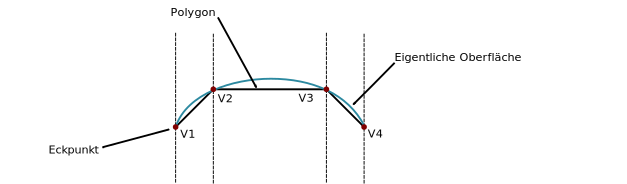
\includegraphics{img/shading_mesh.pdf}
    \caption{Illustration der Ausgangslage\protect\footnotemark}\label{
        fig:shading_mesh_illustration}
\end{figure}
\footnotetext{Eigene Darstellung mittels Inkscape, angelehnt
    an~\cite{hughes_computer_2013}}

Um die Intensität der Farbe für einen Eckpunkt $\bm{V}_{1}$ zu
berechnen, wird der Normalenvektor des Eckpunktes (\textit{vertex
    normal}) benötigt. Es handelt sich dabei um den Normalenvektor der
Oberfläche $\bm{N}$ an der Position des Eckpunktes $\bm{V}_{1}$.

Im Laufe der Zeit wurde die Berechnung der Schattierung so weit
entwickelt, dass sie praktisch ausschliesslich durch Grafikkarte (GPU)
gemacht werden kann.  Man spricht hier vom Begriff ``Shader''. Es
handelt sich dabei mittlerweile um eigene (Grafik-) Applikationen, deren
Zweck weit über die reine Berechnung von Schattierungen hinausgeht. Man
unterscheidet zwischen Shadern für geometrische Berechnungen
(\textit{geometry shaders} oder \textit{vertex shaders}) sowie Shader
für Berechnungen bezüglich Pixeln  oder (Bild-) Fragmenten
(\textit{pixel shaders} oder \textit{fragment
shaders})~\parencite[Kapitel 33]{hughes_computer_2013}.

Der interessierte Leser sei für weitere Details auf~\citetitle[Kapitel
33]{hughes_computer_2013} von~\cite{hughes_computer_2013},
auf~\citetitle{opengl_foundation_rendering_2015}
von~\cite{opengl_foundation_rendering_2015}
sowie~\citetitle{fernando_cg_2003} von~\cite{fernando_cg_2003}
verwiesen.

\subsection{Flat-Shading --- per vertex lighting}
\label{subsec:flat_shading}

% * Calculate normal for each vertice by averaging line-segment normals, e.g.
%   (normal(V1V2) + normal(V3V4)) / 2 to determine per vertex color
%   * Image of calculated normals: line-segment (given through mesh) and vertex
% * One color per face determined by vertex' color

Bei Flat-Shading wird pro Oberfläche (Polygon) ein Eckpunkt $\bm{V}_{1}$
als Schlüssel-Punkt für die Farbe bzw.\ die Intensität bestimmt.
Daraufhin wird die Farbe des Punktes als Farbe für die gesamte
Oberfläche angenommen~\parencite[S. 734]{foley_computer_1996}.

Diese Annahme ist nur unter den folgenden Voraussetzungen gültig~\parencite[S. 734]{foley_computer_1996}:
\begin{enumerate}
    \item{Die zugrundeliegende Lichtquelle befindet sich unendlich weit
            entfernt, so dass der Winkel zwischen dem Normalenvektor der
            Oberfläche $\bm{n}$ und der Lichtquelle $\bm{l}$, also
            $\bm{n}\cdot{}\bm{l}$, für die gesamte Oberfläche konstant
            ist.}
    \item{Der Betrachter befindet sich ebenfalls unendlich weit von der
        Oberfläche entfernt, so dass der Winkel zwischen dem
        Normalenvektor der Oberfläche und dem Betrachter
        $\bm{n}\cdot{}\bm{v}$ für die gesamte Oberfläche konstant ist.}
    \item{Das Polygon ist eine effektive Repräsentation der Oberfläche
            und nicht nur eine Näherung einer runden Oberfläche.}
\end{enumerate}

\begin{figure}[H]
    \centering
    
\includegraphics{img/flat_shading.pdf}
    \caption{Illustration des Flat-Shadings\protect\footnotemark}\label{
        fig:flat_shading_illustration}
\end{figure}
\footnotetext{Eigene Darstellung mittels Inkscape, angelehnt
    an~\cite{hughes_computer_2013}}

Ist eine der ersten beiden Voraussetzungen nicht gegeben, so muss für
den Vektor der Lichtquelle $\bm{l}$ bzw.\ den Vektor des Betrachters
$\bm{v}$ ein konstanter Wert berechnet
werden.~\citeauthor{foley_computer_1996} gibt hier als Beispiele das
Zentrum des Polygones oder den ersten Eckpunkt des Polygones
an~\parencite[S. 735]{foley_computer_1996}.

\subsection{Gouraud-Shading --- face interpolated lighting}
\label{subsec:gouraud_shading}

Bei Gouraud-Shading handelt es sich um ein Shading-Verfahren, welches
die Intensität der Farbe der Eckpunkte von Oberflächen eines
Polygon-Netzes (\textit{Mesh}) interpoliert.

\begin{figure}[H]
    \centering
    \includegraphics{img/gouraud_shading.pdf}
    \caption{Illustration des Gouraud-Shadings\protect\footnotemark.}\label{
        fig:gouraud_shading_illustration}
\end{figure}
\footnotetext{Eigene Darstellung mittels Inkscape, angelehnt
    an~\cite{hughes_computer_2013}}

Um die Farbe eines Eckpunktes von Oberflächen zu berechnen,
schlägt~\citeauthor{gouraud_continuous_1971} in seiner
Arbeit~\citetitle{gouraud_continuous_1971}
von~\citeyear{gouraud_continuous_1971} die Berechnung des
Durchschnittswertes der Normalenvektoren der Oberflächen zweier
adjazenter Liniensegmente (im 2D-Raum) bzw.\  aller adjazenter Dreiecke
(im 3D-Raum) vor~\parencite[S. 92]{gouraud_continuous_1971}.

\begin{figure}[H]
    \centering
    \includegraphics{img/shading_mesh_normals.pdf}
    \caption{Illustration der berechneten Normalenvektoren $\bm{n}_{v_{2}}$ und
    $\bm{n}_{v_{3}}$ an den Eckpunkten $v_{2}$ und $v_{3}$ sowie des
    Normalenvektors $\bm{n}_{v_{23}}$ der Kante $\bm{v_{2}v_{3}}$
    \protect\footnotemark.}\label{fig:gouraud_shading_normals_illustration}
\end{figure}
\footnotetext{Eigene Darstellung mittels Inkscape, angelehnt
    an~\cite{hughes_computer_2013}}

Die Berechnung des Normalenvektors eines Eckpunktes via Durchschnittswert ist
üblicherweise eine genügend gute Näherung an die Oberflächennormale der
eigentlichen Oberfläche. Die Präzision hängt dabei aber eindeutig von der
Granularität des Modelles (\textit{Mesh}) ab.

\subsection{Phong-Shading --- normal interpolated lighting}
\label{subsec:phong_shading}

Phong-Shading ist eine Verbesserung des Gouraud-Verfahrens. Es bietet
eine bessere Annäherung an die Schattierung bzw. Darstellung von glatten
Oberflächen. Das Verfahren ist geeigneter für ein Beleuchtungsmodell,
welches kleine spiegelnde Reflexionen bietet, wie z.B. das
Phong-Beleuchtungsmodell.

Bei Phong-Shading wird ein Normalenvektor linear an einer Oberfläche
(eines Polygons) interpoliert, ausgehend von den Normalenvektoren der
Kanten der Oberfläche (im obigen Beispiel wäre dies
$\bm{n}_{v_{2}v_{3}}$). Die Oberflächennormale wird an jedem Pixel
interpoliert und normalisiert und kommt dann für die Berechnung der
Farbwerte anhand eines Beleuchtungsmodelles, wie zum Beispiel das
Phong-Beleuchtungsmodell, zum Einsatz. Daher ist Phong-Shading viel
rechenintensiver als Gouraud-Shading, da das Beleuchtungsmodell für
jeden Pixel anstatt für jede Kante berechnet werden muss.

\begin{figure}[H]
    \centering
    \includegraphics{img/phong_shading_mesh_normals.pdf}
    \caption{Stark vereinfachte Illustration der interpolierten
        Normalenvektoren anhand der Kante $\bm{v_{2}v_{3}}$
    \protect\footnotemark.}\label{fig:phong_shading_normals_illustration}
\end{figure}
\footnotetext{Eigene Darstellung mittels Inkscape, angelehnt
    an~\cite{hughes_computer_2013}}

\begin{table}[H]
    \centering
    \caption{Vergleich der genannten Shading-Verfahren anhand einer
    Beispielszene\protect\footnotemark.}\label{table:shading_comparision}
    \begin{tabular}{p{0.5\textwidth}p{0.5\textwidth}}
        \toprule
            \textbf{Flat-Shading} &
            \textbf{Gouraud-Shading} \\
        \cmidrule(r){1-1}\cmidrule(lr){2-2}
            \includegraphics[width=0.4\textwidth]{img/flat_shading_example.pdf} \newline &
            \includegraphics[width=0.4\textwidth]{img/gouraud_shading_example.pdf} \newline \\
        \toprule
            \textbf{Gouraud-Shading} \par \textbf{mit Phong-Beleuchtungsmodell} &
            \textbf{Phong-Shading} \par \textbf{mit Phong-Beleuchtungsmodell} \\
        \cmidrule(r){1-1}\cmidrule(lr){2-2}
            \includegraphics[width=0.4\textwidth]{img/phong_gouraud_shading_example.pdf} \newline &
            \includegraphics[width=0.4\textwidth]{img/phong_phong_shading_example.pdf} \newline \\
        \bottomrule
    \end{tabular}
\end{table}
\footnotetext{\cite{brian_danchilla_beginning_2014}}
